\documentclass{report}
\usepackage{snepospec}
% TODO add snepo document imports

\begin{document}
\setlength{\headsep}{16pt}
\chead{Depot Users Guide}

\chapter{Depot, can it bake bread?}

\paragraph{}
\textbf{Depot} allows you as a Flash or Javascript developer to create
rich internet applications without using PHP, ASP, or any other
three-lettered server side scripting language. This is because Depot
works entirely over HTTP which, incidentally, both Flash and
Javascript are quite good at.

\paragraph{}
What exactly can you do with Depot? Some examples are: 
\begin{itemize}
\item Write a guestbook for your blog
\item Write that blog so you can write a guestbook
\item Write a peachy keen wiki
\item Write a high score table, a chat room...
\item You get the picture, anywhere that you would use a database for
  a web application you can probably use Depot
\end{itemize}

\paragraph{}
The gist of it is that you shouldn't have to know anything about
databases or server side programming to write a guestbook. However,
when you want to scale your project up Depot is right there offering
the ability to easily store millions of records and retrieve them
faster than your dear aunt Hortense can shoot dirty looks at ruffians.


\section{Getting Started}
\subsection{Windows}
\begin{itemize}
\item Double click the \texttt{depot-VERSION.exe} file. This will start the
  Depot installer. Follow the on screen instructions.
\item Click \texttt{Start$\rightarrow$All Programs$\rightarrow$Snepo$\rightarrow$Depot$\rightarrow$start-web}
\item Click \texttt{Start$\rightarrow$All Programs$\rightarrow$Snepo
$\rightarrow$Depot$\rightarrow$start-depot-service}
\end{itemize}

\subsection {Mac}
\begin{itemize}
\item Open the \texttt{depot-VERSION.pkg} file. This will start the
  Depot installer. Follow the instructions, Depot will be installed
  under \texttt{/Users/YourName/depot}.
\item Open a terminal window
\item \texttt{cd path/to/depot}
\item \texttt{./start-web.sh \&}
\item \texttt{./start-depot.sh}
\end{itemize}

\subsection{Linux}
\begin{itemize}
\item \texttt{tar -xzvf depot.tar.gz}
\item \texttt{cd depot}
\item \texttt{./start-web.sh \&}
\item \texttt{./start-depot.sh}
\end{itemize}

When depot starts it examines the \texttt{depot.config}
file. The admin password is set using the value of the
\texttt{admin-password} parameter. Any user who is authenticated 
as an admin has unrestricted access to your Depot data store.
The default password is \texttt{cthulu}. If you change the password
in the config file restart Depot to load the new password.
We recommend changing the password before deploying to any public server.

\paragraph{}
If you want to make sure that you've properly set things up, after
depot is started point your browser at
\url{http://localhost:2323/depot/junk}. If things are working
correctly you will see a bunch of output like this:

\begin{center}
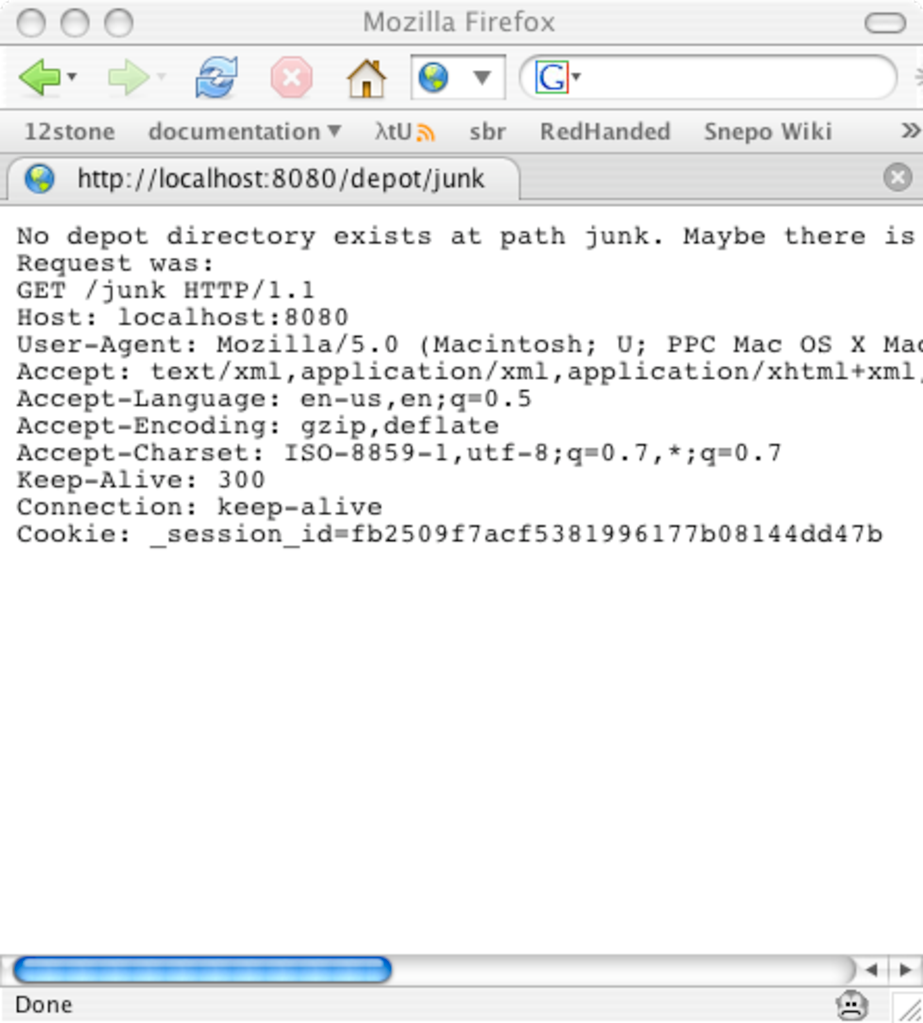
\includegraphics[scale=0.70]{wiki-tutorial-images/wiki-screenshot-404.pdf}
\end{center} 

\paragraph{}
Note that if you are using FireFox the output may not display in the
browser but you will be prompted to download a text file. 

\chapter{What is a Depot client? And what, exactly \textit{is}
  Depot? }

\paragraph{}
Depot itself is a server, it handles incoming requests, does some
magic and then responds. The requests come from a Depot client, we
provide both a Flash and a Javascript client for Depot. The clients
communicate over HTTP which is the same protocol that web browsers
use. In fact if you open a Depot URL in a web browser it will display
a Depot response.

\paragraph{}
Depot exists to store data, be it a blog entry, a forum post, a high
score, or your extensive muffin recipe collection. The things that you
can do with Depot data are: 

\snepolistbox{
  \item GET - Retrieve data from Depot
  \item PUT - Save or update data in Depot
  \item DELETE - Remove data from Depot
}

\paragraph{}
Depot puts data into \textbf{directories}. This is an integral part of
how Depot works, it also happens to be very similar to how the
internet is already set up. Funny that. Here's a comparison of a
normal URL with a Depot URL.
\begin{verbatim}
http://depot.snepo.com/pandasausage/
\end{verbatim}
and a Depot URL:
\begin{verbatim}
http://depot.snepo.com:2323/pandasausage/
\end{verbatim}
The difference is that the port number (after the colon in the URL) is
2323. This is the default for Depot, it means that you can run a
webserver and an instance of Depot on the same machine without them
interfering with each other. Both the web URL and the Depot URL
represent \textbf{directories}. From a web URL you generally get HTML
pages and from a Depot URL you can get your data.
\paragraph{}
Each entry in a Depot directory is automatically assigned an id. This
id is used to identify the entry in the directory uniquely. To request
an entry individually you use a URL variable:
\begin{verbatim}
http://depot.snepo.com:2323/pandasausage?id=23
\end{verbatim}

That's enough to give a quick overview of what Depot is. If you want
to go deeper into the greasy, grimy gopher guts of Depot the entire
API is published online along with information on building custom
clients. If you want to just get started and create data driven
applications then you can move right on to integrating Depot with
Flash or Javascript.

\paragraph{}
Lastly, our philosophy with Depot clients is to keep them open and
free. That means that if you want to tinker with the source code or
write and distribute your own client software for Depot you are free
to do so.

\chapter{The Javascript Client}


\paragraph{}
The Javascript client takes advantage of the wonderful Prototype
Javascript library\footnote{Available free and open source from
  http://prototype.conio.net} to provide the boilerplate code for Ajax
functionality. There is a quick start tutorial
(\texttt{wiki-tutorial.pdf}) in the docs directory of your Depot
install that will take you through the steps necessary to write a wiki
in 30 minutes or less.
\paragraph{}
To use the client you must include both the
\texttt{prototype-1.4.0.js} file and the \texttt{depot-client.js} file
in your HTML page.
\begin{Verbatim}[frame=single]
<html>
  <head>
    <script language="javascript" 
            src="../lib/prototype-1.4.0.js"></script>
    <script language="javascript" 
            src="../lib/depot-client.js"></script>
  </head>
  <body>

  </body>
</html>
\end{Verbatim}

Depot directories are managed through instances of
\texttt{Depot.Object}'s. When you are using Javascript all Depot
directory names must begin with \texttt{/depot/}\footnote{This is
  because Depot needs to be proxied in order to interact with
  Javascript. This is explained later in the user guide}

\begin{Verbatim}[frame=single]
 var ps = new Depot.Object("/depot/pandasausage");
\end{Verbatim}

The above binds a \texttt{Depot.Object} to a directory named
\texttt{/depot/pandasausage}. 

\begin{Verbatim}[frame=single]
 ps.onCreate = weMadeAPandaSausageDirectory;

 function weMadeAPandaSausageDirectory(dat,res) {
   alert("New Panda Sausage!");
 }

 ps.newDirectory();
\end{Verbatim}
\paragraph{}
Each action that a \texttt{Depot.Object} performs can have an event
handler assigned to it. In this case the \texttt{onCreate} event was
set to trigger a function that alerts us of the new panda sausage
directory.

\paragraph{}
Event handling functions need to accept two arguments, the body of the
response (which in the case of a \texttt{get} request will be parsed
XML) and the raw HTTP Response.

\section{The Depot.Object Commands and Events}

\paragraph{NOTE} All of the \texttt{Depot.Object} commands take an
optional argument that is a collection of overrides. This argument
comes after the standard arguments in the function (e.g. in
\texttt{get} it is the second argument but in \texttt{findAll} it is
the first). These options are in the format: 

\begin{Verbatim}[frame=single]
  var opts = {onCreate: customHandler};
  ps.newDirectory(opts);
\end{Verbatim}

The above would call the \texttt{customHandler} handler rather than
the \texttt{weMadeAPandaSausageDirectory} handler when the
\texttt{newDirectory} command was complete.

\subsection{Depot.Object Commands}

\subsubsection{newDirectory}
\paragraph{}
Creates a new Depot directory. This will return a Conflict error
if the directory already exists.

\begin{Verbatim}[frame=single]
 ps.newDirectory();
\end{Verbatim}

\paragraph{}
\textit{Event \texttt{onCreate}}

\subsubsection{restoreDirectory}
\paragraph{}
Restores a deleted depot directory to the state it was in when the
\texttt{removeDirectory} function was called on it. Only directories
that have been \textbf{removed} can be restored. 

\begin{Verbatim}[frame=single]
 ps.restoreDirectory();
\end{Verbatim}

\paragraph{}
\textit{Event \texttt{onCreate}}


\subsubsection{create}
\paragraph{}
Creates an entry in a Depot directory. It takes a string as an
argument and will throw an error if the directory doesn't exist.

\begin{Verbatim}[frame=single]
 var data = "some text";
 ps.create(data);
\end{Verbatim}

\paragraph{}
\textit{Event \texttt{onCreate}}


\subsubsection{update}
\paragraph{}
Updates an entry in a Depot directory. It takes an id and a string as
arguments. If the id doesn't exist in the directory a new entry will
be created using the passed id.

\begin{Verbatim}[frame=single]
 var data = "some text";
 var id   = 23;
 ps.update(id,data);
\end{Verbatim}

\paragraph{}
\textit{Event \texttt{onCreate}}


\subsubsection{get}
\paragraph{}
Retrieves an entry from a Depot directory. Takes an id as an argument.
\begin{Verbatim}[frame=single]
 var id = 1;
 ps.get(id);
\end{Verbatim}

\paragraph{}
\textit{Event \texttt{onGet}}

\subsubsection{getAll}
\paragraph{}
Retrieves all entries and sub-directories from a Depot directory.
\begin{Verbatim}[frame=single]
 ps.getAll();
\end{Verbatim}

\paragraph{}
\textit{Event \texttt{onGet}}


\subsubsection{getFirst}
\paragraph{}
Retrieves the first entry put into a directory.
\begin{Verbatim}[frame=single]
 ps.getFirst();
\end{Verbatim}

\paragraph{}
\textit{Event \texttt{onGet}}

\subsubsection{getLast}
\paragraph{}
Retrieves the last entry put into a directory.
\begin{Verbatim}[frame=single]
 ps.getLast();
\end{Verbatim}

\paragraph{}
\textit{Event \texttt{onGet}}

\subsubsection{getRange}
\paragraph{}
Retrieves entries between two id values from \textit{n} to \textit{n}.
\begin{Verbatim}[frame=single]
 ps.getRange(2,5); // retrieves entries 2,3,4,5
\end{Verbatim}

\paragraph{}
\textit{Event \texttt{onGet}}

\subsubsection{size}
\paragraph{}
Takes no arguments and returns the number of entries in a directory
\begin{Verbatim}[frame=single]
 ps.size(); 
\end{Verbatim}

\paragraph{}
\textit{Event \texttt{onGet}}

\subsubsection{remove}
\paragraph{}
Deletes an entry for a given id. This is not a reversible operation.
\begin{Verbatim}[frame=single]
 var id = 23;
 ps.remove(id);
\end{Verbatim}

\paragraph{}
\textit{Event \texttt{onDelete}}

\subsubsection{removeDirectory}
\paragraph{}
Deletes a directory at a given path. For all intents and purposes the
directory will cease to exist. However, it may be restored by calling
\texttt{restoreDirectory} if necessary.
\begin{Verbatim}[frame=single]
 var path = "/depot/cheesehands";
 ps.deleteDirectory(path);
\end{Verbatim}
\paragraph{}
\textit{Event \texttt{onDelete}}


\subsubsection{destroyDirectory}
\paragraph{}
Irreversibly destroys a directory and all of its content.
\begin{Verbatim}[frame=single]
 var path = "/depot/cheesehands";
 ps.destroyDirectory(path);
\end{Verbatim}
\paragraph{}
\textit{Event \texttt{onDelete}}


\subsubsection{executeQuery}
\paragraph{}
Executes a query directly on a Depot directory. The first argument is
the URL of the query plus an optional query string.
\begin{Verbatim}[frame=single]
 var path = "/depot/squirreljams";
 var qstr = "?id=23";
 ps.executeQuery(path + qstr);
\end{Verbatim}

\paragraph{}
\textit{Event \texttt{onGet}, \texttt{onCreate}, or \texttt{onDelete}}

\subsection{Depot.Object Events}
\paragraph{}
The results of the above method calls will trigger events. Event
handlers are assigned to a \texttt{Depot.Object} in two ways.

\snepolistbox {
 
\item By setting them as defaults
\item By using overrides 

}
\paragraph{}
A default is set by assigning a function to the event on a \texttt{Depot.Object}

\begin{Verbatim}[frame=single]
 var d      = new Depot.Object("/depot/pickled/sausage");
 d.onGet    = function() {alert("Flummoxed beavers!");}
 d.onDelete = porkSausageDeleteHandler;
\end{Verbatim}

Overrides are passed when commands are invoked: 
\begin{Verbatim}[frame=single]
 d.getFirst({onGet: flummoxOverride, onServerError: dieHorribly});
\end{Verbatim}

The available events are: 


\snepolistbox {
\item \texttt{onGet}  a \texttt{get} command is
  successful 

\item \texttt{onCreate} a new object was created (either
  a directory or an entry in a directory)

\item \texttt{onDelete} an object was removed or destroyed

\item \texttt{onNotFound} an action couldn't be completed because the
  directory or object does not exist.

\item \texttt{onServerError} an error has occurred on the depot server.

\item \texttt{onException} an error has occurred inside Javascript code.

 }

\pagebreak
\subsection{The Depot Response Object}

On a get request the depot javascript client either returns a single
response object or an array of them depending on whether the result
contains a single item or multiple items.
\paragraph{}
The object has the following properties

\snepolistbox{

\item Meta Data, all of the meta data about the object is transformed
  into properties named for the camel-cased tag that they corrospond
  to. E.g. \texttt{object-name} becomes \texttt{objectName}.

\item \texttt{data} contains the value of the \texttt{<data />} tag in
  the response, this is null if the request was for meta data only or
  if the item is a \texttt{sub-directory}


\item \texttt{isDirectory} true if the item is a \texttt{sub-directory}.

}

\paragraph{}
An example:

\begin{Verbatim}[frame=single]
var beavers = new Depot.Object("/alien/beaver");
beavers.getAll({onGet: openBeaver});
function openBeaver(dat, res) {
  if(dat.each) {
    dat.each(function(beaver) {
      handleBeaver(beaver);
    });
  } else {
      handleBeaver(beaver);
  }
}
function handleBeaver(beaver) {
    if(beaver.isDirectory) {
       alert("Got a subdirectory of /alien/beaver");
    } else { // it's an alien beaver!
       alert("This beaver was created on " + beaver.creationDate);
       alert("We opened it up to find: " + beaver.data);
    } 
}
\end{Verbatim}

It can get tedious to check for the response all the time. That's why
we included the convenience function \texttt{handleResponse} to
automate the process. Thus \texttt{openBeaver} could be rewritten as
follows:

\begin{Verbatim}[frame=single]
function openBeaver(dat,res) {
  handleResponse(handleBeaver, dat);
}
\end{Verbatim}

\chapter{The Flash Client}

\paragraph{}
The Flash client ..... 
 There is a quick start tutorial
(\texttt{flash-tutorial.pdf}) in the docs directory of your Depot
install that will walk you through building a Flash comments application.

\section{Flash Commands and Events}

\paragraph{}
To use the client you must include the
\texttt{com} directory with your Flash application.
\begin{Verbatim}[frame=single]
import com.snepo.depot.*;
\end{Verbatim}

When you are using Depot behind a webserver
directory names must begin with \texttt{/depot/}\footnote{This is
  because Depot needs to be proxied in order to interact with
  Flash. This is explained later in the user guide}


\subsection{Flash Commands}

\subsubsection{newDirectory}
\paragraph{}
Creates a new Depot directory. This will return a Conflict error
if the directory already exists.

\begin{Verbatim}[frame=single]
 var url = "/dir/subdir";
 PO.newDirectory(url);
\end{Verbatim}

\paragraph{}
\textit{Event \texttt{onCreateDirectory}}

\subsubsection{create}
\paragraph{}
Creates an entry in a Depot directory with optional parameters for name, user defined type (ctype) and id. The command will throw an
error if the directory doesn't exist. The new entry object can be any 
native Flash object (e.g. Number, Boolean, Date, XML etc).

\begin{Verbatim}[frame=single]
 var url = "/dir/subdir";
 var obj = {user:"userName", score:2345}; 
 var name =  "high score"; 
 var ctype = "game score"; 
 var id = 1; 
 PO.create(url, obj, name, ctype, id);
\end{Verbatim}

\paragraph{}
\textit{Event \texttt{onCreate}}

\subsubsection{get}
\paragraph{}
Retrieves an entry data or entry metadata from a Depot directory. 
Meta set to true will only return the metadata for entries. See notes in id expressions later in this chapter.

\begin{Verbatim}[frame=single]
 var url = "/dir/subdir";
 var id = 1; 
 var meta = false; 
 PO.get(url, id, meta);
\end{Verbatim}

\paragraph{}
\textit{Event \texttt{onGet}}

\subsubsection{getFirst}
\paragraph{}
Retrieves the first entry put into a directory. 
Meta set to true will only return the metadata for entries.

\begin{Verbatim}[frame=single]
 var url = "/dir/subdir";
 var meta = false;
 PO.getFirst(url, meta);
\end{Verbatim}

\paragraph{}
\textit{Event \texttt{onGet}}

\subsubsection{getLast}
\paragraph{}
Retrieves the last entry put into a directory. 
Meta set to true will only return the metadata for entries.

\begin{Verbatim}[frame=single]
 var url = "/dir/subdir";
 var meta = false;
 PO.getLast(url, meta);
\end{Verbatim}

\paragraph{}
\textit{Event \texttt{onGet}}

\subsubsection{remove}
\paragraph{}
Deletes a directory at a given path. For all intents and purposes 
the directory will cease to exist. However, it may be restored by 
calling restore if necessary. If an id is supplied an entry
is deleted. This is not a reversible operation.

\begin{Verbatim}[frame=single]
 var url = "/dir/subdir";
 var id = 1; // entry id or expression (not required when removing dir)
 PO.remove(url, id);
\end{Verbatim}

\paragraph{}
\textit{Event \texttt{onDelete}}

\subsubsection{destroy}
\paragraph{}
Irreversibly destroys a directory and all of its content.

\begin{Verbatim}[frame=single]
 var url = "/dir/subdir";
 PO.destroy(url);
\end{Verbatim}

\paragraph{}
\textit{Event \texttt{onDelete}}

\subsubsection{restore}
\paragraph{}
Restores a deleted depot directory to the state it was in 
when the remove function was called on it. Only directories 
that have been removed can be restored.

\begin{Verbatim}[frame=single]
 var url = "/dir/subdir";
 PO.restore(url);
\end{Verbatim}

\paragraph{}
\textit{Event \texttt{onGet}}

\subsubsection{destroyAuthentication}
\paragraph{}
Destroys persistent authentication data.

\begin{Verbatim}[frame=single]
 PO.destroyAuthentication();
\end{Verbatim}

\paragraph{}
\textit{Event \texttt{none}}

\subsubsection{authorize}
\paragraph{}
Authorize a user with username and password.

\begin{Verbatim}[frame=single]
 var username = "gary";
 var password = "password123"
 PO.authorize(username, password);
\end{Verbatim}

\paragraph{}
\textit{Event \texttt{none}}

\subsubsection{getPermissions}
\paragraph{}
Gets the directory permissions for a single user. 
Note: Entry specific permissions have not been implemented (yet ;]).

\begin{Verbatim}[frame=single]
 var id = null;
 var url = "/dir/subdir";
 var username = "gary";
 PO. getPermissions(url, id, username);
\end{Verbatim}

\paragraph{}
\textit{Event \texttt{onGet}}

\subsubsection{putPermissions}
\paragraph{}
Saves the directory permissions for a single user.
The permission string is a combination of 'c' for create, 
'r' for retrieve, 'u' for update and 'd' for delete (crud).
Note: Entry specific permissions have not been implemented (yet ;]).

\begin{Verbatim}[frame=single]
 var url = "/dir/subdir";
 var id = null;
 var username = "gary";
 var permissions = "crd"
 PO. putPermissions(url, id, username, permissions);
\end{Verbatim}

\paragraph{}
\textit{Event \texttt{onCreate}}

\subsubsection{putUser}
\paragraph{}
Creates a new user with password.

\begin{Verbatim}[frame=single]
 var username = "gary";
 var password = "password123"
 PO.putUser(username, password);
\end{Verbatim}

\paragraph{}
\textit{Event \texttt{onCreate}}


\subsection{Flash Events}
\paragraph{}
The Depot Flash client contains setter methods for the various Depot events. Handlers are applied using the following syntax:

\begin{Verbatim}[frame=single]
 customEventHandler = function() {
	// your handler AS code goes here
};
 PO.onEvent = customEventHandler;
\end{Verbatim}

Note: the use of the \textit{this} keyword within a custom event handler script block refers to the instance of Depot that is broadcasting the event. The following handlers are available:

\subsubsection{onCreateDirectory}
Event: Triggered upon the succesful creation of a new directory.
Returns: the newly created directory path.
\subsubsection{onCreate}
Event: Triggered upon the succesful creation of a new entry.
Returns: an id for the created entry.
\subsubsection{onGet}
Event: Triggered upon the successful retrieval of an entry, entries, metadata or directory.
Returns: an array of entries, an array of metadata (if requested) and an array of directories;

\begin{Verbatim}[frame=single]
 customOnGet = function(responseAr, metadataAr, directoryAr) {
	// your code here
};
 PO.onEvent = customOnGet;
\end{Verbatim}

\subsubsection{onDelete}
Event: Triggered upon the successful deletion of an entry of directory.
Returns: Returns a message "Deleted Entry" or "Deleted Directory \textit{directory}"
\subsubsection{onError}
Event: Triggered upon error
Returns: an error message string and an error code.
See section on error handling for more information.

\subsubsection{onConnect}
Event: Triggered upon connecting to a Depot server.
Returns: Connection status boolean.

\subsection{Other Depot Methods}
There are other of setters and methods that allow for easier debugging and authentication:

\subsubsection{debug}
Setter method for turning debugging on. While debug is true request and response data is traced to the IDE output window.

\begin{Verbatim}[frame=single]
 PO.debug = true;
\end{Verbatim}

\subsubsection{connectionState}
Returns the state of the socket connection. The client connection to Depot is not persistent so the connectionState property can be used to monitor for connection timeouts.

\begin{Verbatim}[frame=single]
 trace(PO.connectionState);
\end{Verbatim}






\section{Flash Error Handling}
\paragraph{}
The Depot client has internal error messaging that will respond with common error types. When building your Flash application it is wise to include a custom error handler to trap any Depot error and to respond accordingly. Custom error handlers are implemented in the same way as all other event handlers:

\begin{Verbatim}[frame=single]
 customOnError = function(msg, code) {
	// your code here
};
 PO.onError = customOnError;
\end{Verbatim}

An error reference class is installed with the Depot client and can be used to reference error codes by their static string representations:

\begin{Verbatim}[frame=single]
import com.snepo.depot.Errors
// depot instantiation code
 customOnError = function(msg, code) {
	if(code == Errors.NOT_FOUND) {
		// handle NOT_FOUND error
	}
};
 PO.onError = customOnError;
\end{Verbatim}




\section{Flash Query Expressions}
For the time being the only permitted variable in the URL string is
"id" (e.g. /a/path?id=1). The value of the variable may be expressed
as a scalar value (e.g. the literal 1) or as an expression. Valid
expressions are:

\subsubsection{Range Query}
\begin{Verbatim}[frame=single]
/a/path?id=1..3 returns records with id equal to 1,2, and 3 
/a/path?id=1.. returns all records >= 1 
/a/path?id=..3 returns all records <= 3 
\end{Verbatim}
\subsubsection{Min/Max Query}
\begin{Verbatim}[frame=single]
/a/path?id=(min) returns the first record (the lowest id value) 
/a/path?id=(max) returns the last record (the highest id value) 
\end{Verbatim}
\subsubsection{Comma Delimited Query}
\begin{Verbatim}[frame=single]
/a/path?id=1,4..6,(max) returns ids of 1, 4 through 6, and the max id 
\end{Verbatim}
\paragraph{}


\chapter{Depot Explorer}

\paragraph{}
The Depot Explorer is your gooey, GUI interface to the Depot server.
It can run as a stand alone application or inside the Flash IDE. To
install the Flash IDE panel double click \texttt{depot.mxp}. Depot
Explorer can access both local and remote Depot data stores. That
means that you can keep track of your deployed Depot instances as well
as those that are local to your machine without jumping though any
hoops.

\section{Running Depot Explorer}
\subsubsection{Windows}
Click \texttt{Start$\rightarrow$All
  Programs$\rightarrow$Snepo$\rightarrow$Depot$\rightarrow$Depot
  Explorer}

\subsubsection {Mac}
Double click the \texttt{"Depot Explorer.hqx"} file. Depot Explorer will 
be installed under the \texttt{flash} directory.

\subsubsection{Linux}
The Linux version of Depot is for deployment to web servers. Since it
is not meant to be used in a desktop capacity there is no version of
Depot Explorer. However, when Flash Player support improves we will
provide one.

\section{Add Depot Instance}
\begin{center}
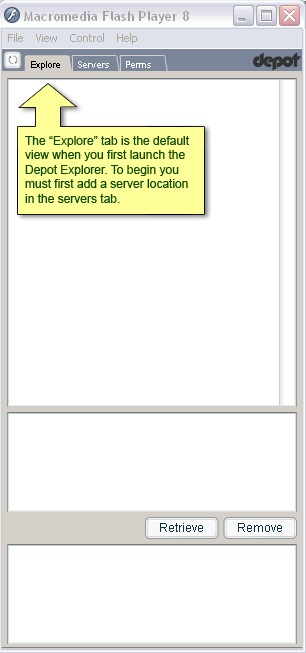
\includegraphics[scale=0.5]{users-images/Step1-annotated.png}
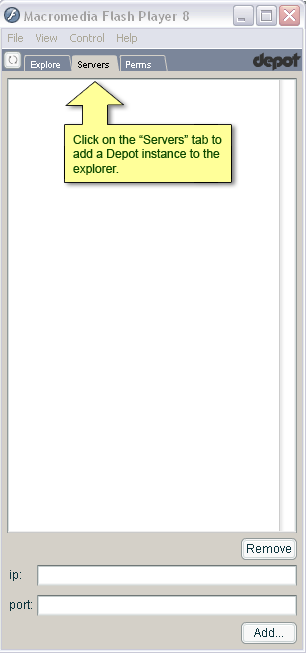
\includegraphics[scale=0.5]{users-images/Step2-annotated.png}
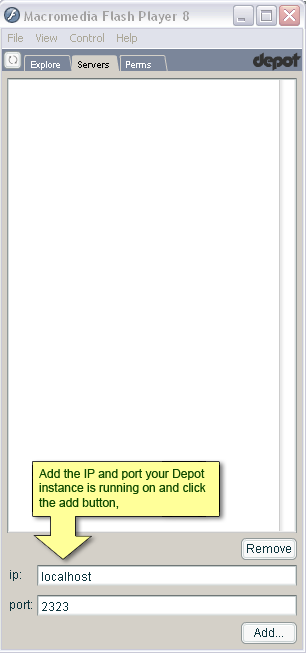
\includegraphics[scale=0.5]{users-images/Step3-annotated.png}
\end{center}

\section{Browse Depot Data}
\begin{center}
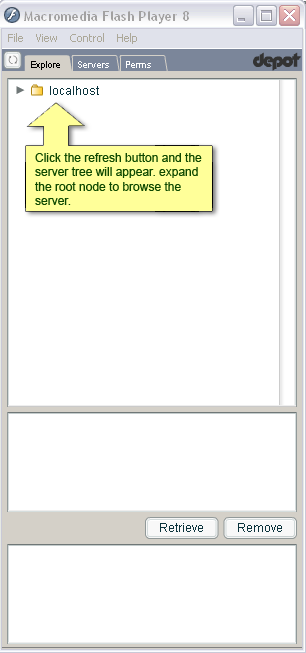
\includegraphics[scale=0.5]{users-images/Step5-annotated.png}
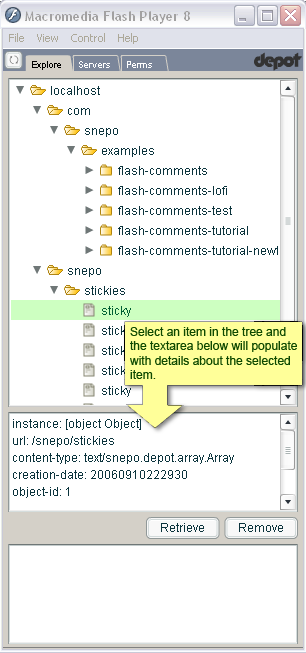
\includegraphics[scale=0.5]{users-images/Step6-annotated.png}
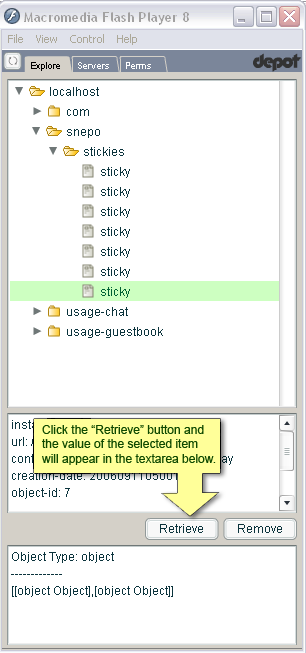
\includegraphics[scale=0.5]{users-images/Step7-annotated.png}
\end{center}

\section{Edit User Permissions}
\begin{center}
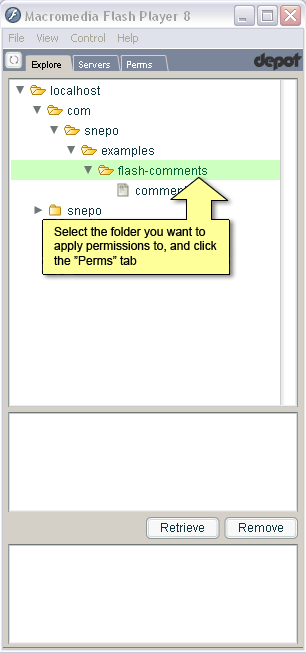
\includegraphics[scale=0.5]{users-images/Step8-annotated.png}
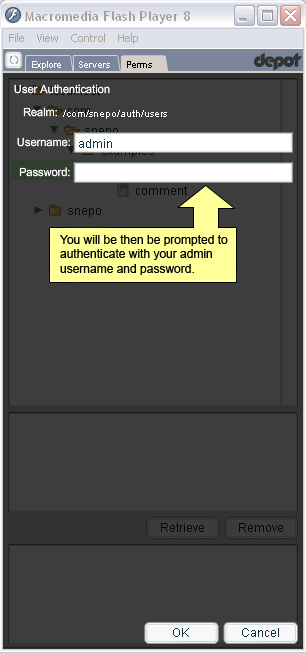
\includegraphics[scale=0.5]{users-images/Step9-annotated.png}
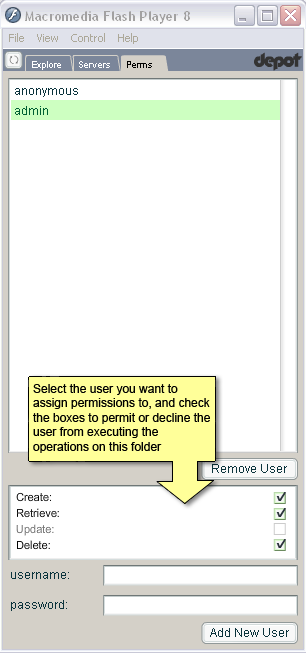
\includegraphics[scale=0.5]{users-images/Step10-annotated.png}
\end{center}

\section{Add New User}
\begin{center}
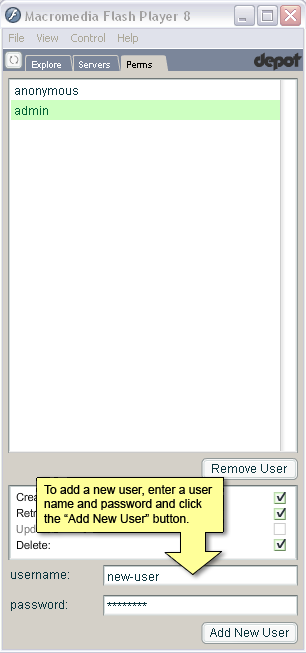
\includegraphics[scale=0.5]{users-images/Step11-annotated.png}
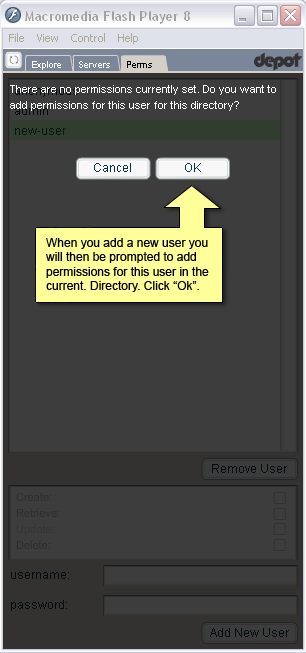
\includegraphics[scale=0.5]{users-images/Step12-annotated.png}
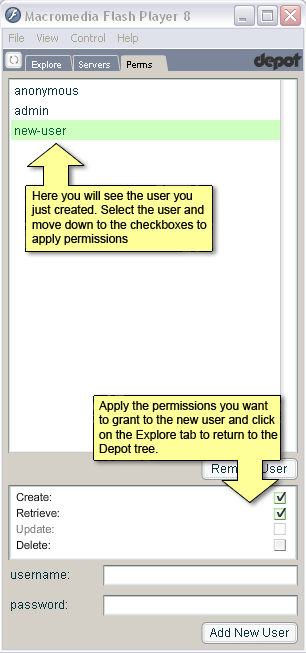
\includegraphics[scale=0.5]{users-images/Step13-annotated.png}
\end{center}


\chapter{Proxying}
\paragraph{}
Javascript (and Flash without a policy file) does not allow you to
make HTTP requests to different domains or different ports on the same
domain. Not to worry, like a giant marsupial Depot is lurking just
around the corner with a solution and a furry pouch.
\paragraph{}
The solution is \textbf{proxying}. The web server maps a request to
URLs matching a certain pattern to a different location. The
development server (depot-http) that comes with the Depot install does
this for you. All requests aimed at urls starting with
\texttt{/depot/} are remapped to port 2323.

\begin{Verbatim}[frame=single]
http://localhost:8080/depot/monkey/houseplant
\end{Verbatim}

Becomes 

\begin{Verbatim}[frame=single]
http://localhost:2323/monkey/houseplant
\end{Verbatim}

\paragraph{}
And nobody is any the wiser. Production web servers like
Apache\footnote{http://apache.org} can be configured to proxy requests
quite easily. Information on setting up Apache to proxy is available
at the \url{http://depot.snepo.com} website. For development the
provided depot-http web server should be just fine for all of your
proxying needs.

\paragraph{Important!} When Depot receives a request that is prefixed
with \texttt{/depot} it internally removes that part of the URL. In
other words even though you might create a directory called
\texttt{/depot/aqua/bear} it will really create the directory
\texttt{/aqua/bear}. 

\paragraph{}
For those of you who would like to deploy to IIS a proxy module is
under development and will be available very soon. Check the Depot
website for updates on its progress.


\begin{appendices}
\chapter{The Depot Response XML Format}


\paragraph{}
When a result is returned from a depot GET request it will come in XML
format. 
\begin{Verbatim}[frame=single]
<?xml version="1.0"?>
<depot-result>
  <directory>
    <meta-data>
      <object-name>com/snepo/cthulu/bicycle</object-name>
      <entries>1</entries>
      <description>depot directory</description>
    </meta-data>
  </directory>
  <entry>
    <meta-data>
      <owner>Hagbard Celine</owner>
      <object-name>Bicycle Rhubarb</object-name>
      <object-id>1</object-id>
      <creation-date>20060724</creation-date>
      <content-type>text/plain</content-type>
    </meta-data>
    <data><![CDATA[RHUBARB DATA]]></data>
  </entry>
</depot-result>
\end{Verbatim}

\subsection{XML Tags}

\subsubsection{directory}
\paragraph{}
This tag only comes back on a directory contents query. It contains
information about the directory that was requested. E.g. a query for
/com/snepo/cthulu/bycicle would return the above \texttt{<directory>}
response.

\subsubsection{metadata}
Information about data in a result set. If the metadata occurs inside
an \texttt{<entry>} tag it will contain the sort of information you
would expect to find in a normal file system such as the owner of the
data, it's creation date, etc... Inside a directory tag it contains
the directory name and number of entries.

\subsubsection{object-name}
This corresponds to a file name. When referring to a directory it is
the URL of the directory (without the hostname). When it is regarding
an entry it is the name of that particular entry and does not need to be unique.

\subsubsection{entries}
The number of entries contained by a directory

\subsubsection{description}
A description of the type of item returned

\subsubsection{object-id}
Only present in \texttt{<entry>} tags, this is the unique identifier
for this object in this directory.

\subsubsection{creation-date}
The date that an item was created in the format \textit{YYYYMMDD}.

\subsubsection{content-type}
The mime type of the entry. Usually a text/ or xml/ prefixed value.

\subsubsection{data}

The information stored under an entry. If the information has been
stored as raw data it will be surrounded by a \texttt{<![CDATA[]]>}
tag. If it stored as XML it will simply be a child node of
\texttt{<data>}


\chapter{The Javascript API Table}
\begin{center}
\setlength{\extrarowheight}{6pt}
\begin{tabular*}{0.75 \textwidth}
      {@{\extracolsep{\fill}}|l|l|l|}
\hline
\textbf{Function Name} & \textbf{Arguments} & \textbf{Events} \\
\hline
        newDirectory     & opts*               & onCreate \\
        restoreDirectory & path, opts*         & onCreate \\
        create           & data, opts*         & onCreate \\
        update           & id, data, opts*     & onCreate \\
\hline
        get              & id, opts*           & onGet \\
        getAll           & opts*               & onGet \\
        getFirst         & opts*               & onGet \\
        getLast          & opts*               & onGet \\
        getRange         & from, to, opts*     & onGet \\
        size             & opts*               & onGet \\
\hline
        delete           & id, opts*           & onDelete \\
        deleteDirectory  & path, opts*         & onDelete \\
        destroyDirectory & path, opts*         & onDelete \\
\hline
        executeQuery     & path, opts*         & onGet, onCreate, or onDelete \\
\hline
        \multicolumn{3}{|c|}{arguments marked * are optional.} \\
\hline
\end{tabular*}
\end{center}
\chapter{The Flash API Table}
\begin{center}
\setlength{\extrarowheight}{6pt}
\begin{tabular*}{0.75 \textwidth}
      {@{\extracolsep{\fill}}|l|l|l|}
\hline
\textbf{Function Name} & \textbf{Arguments} & \textbf{Events} \\
\hline
        newDirectory     & url                & onCreateDirectory \\
        create           & url, obj, name*, ctype*, id*    & onCreate \\
        putUser          & username, password & onCreate \\
        putPermissions   & url, username, permissions & onCreate \\

\hline
        get              & url, id*, meta*    & onGet \\
        getFirst         & url                & onGet \\
        getLast          & url                & onGet \\
        restore          & url                & onGet \\
        getPermissions   & url, username      & onGet \\

\hline
        remove           & url, id*           & onDelete \\
        destroy          & id, opts*          & onDelete \\

\hline
        \multicolumn{3}{|c|}{arguments marked * are optional.} \\
\hline
\end{tabular*}
\end{center}

\end{appendices}

\end{document}
